\begin {document}

\title {\ZHH \huge 从手机到internet}
\author {\small gaccob}
\date {\small 2014 年 1 月 3 日}
\maketitle
\begin {center}
{\ZHH \small 标签: 4g, internet, lte, 手机, 骨干网}
\end {center}

\vspace {10pt}
\section {\ZHH 手机到internet之间的数据传输} {
    \begin {figure} [htbp]
        \centering
        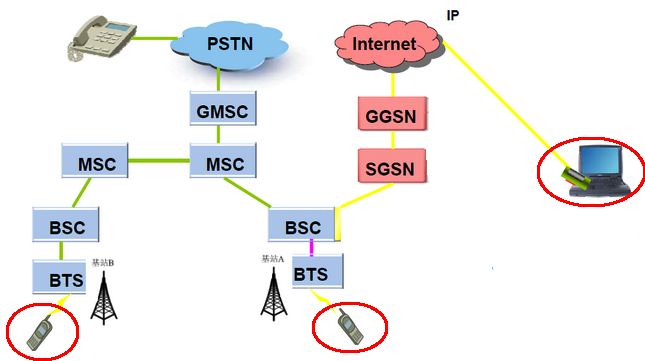
\includegraphics [width=400pt, keepaspectratio] {transfer.png}
    \end {figure}

    \begin {itemize}
        \item { \textcolor {blue} {基站收发台BTS(Base Transceiver Station) } } \\
        { 由BSC控制, 服务于某个小区的无线收发信设备, 完成BSC与无线信道之间的转换, 实现BTS和移动台之间通过空中接口的无线传输及相关的控制功能. } \\
        { BTS和移动终端(专业术语叫做移动台, MS)之间的是\textcolor{blue}{Um接口}, 也称空中接口, 在GSM/GPRS/EDGE网络中, 传输MS与网络之间的信令信息和业务信息. } \\

        \item { \textcolor {blue} {基站控制器BSC(Base Station Control)} } \\
        { BSC在基站子系统中起控制器和话务集中器作用, 一个基站控制器根据话务量可以控制数十个BTS. } \\
        { BTS和BSC之间是\textcolor{blue}{Abis接口}: 遵循GSM规范08.5X系列要求, 在Abis接口上BSC提供BTS配置, BTS监测, BTS测试及业务控制等信令控制信息. } \\

        \item { \textcolor {blue} {基站子系统BSS} } \\
        { 可以由一个BSC和多个BTS组成, BSC根据业务量, 可以控制多个BTS. BTS负责传输, BSC负责管理和控制. } \\

        \item { \textcolor {blue} {移动业务交换中心MSC(mobile switching center)} } \\
        { MSC是网路的核心, 它提供交换功能以及面向系统其他功能实体. MSC可以从三种数据库(HLR, VLR, AUC)获取处理用户位置登记和呼叫请求所需的全部数据. 反之, MSC也根据其最新获取的信息请求更新数据库的部分数据. MSC具有号码储存译码, 呼叫处理, 路由选择, 回波抵消, 超负荷控制等功能; MSC作为网路核心, 应能支持位置登记, 越区切换和自动漫游等移动管理功能; MSC还应支持信道管理, 数据传输, 以及包括鉴权, 信息加密, 移动台设备识别等安全保密功能. } \\

        \item { \textcolor {blue} {网关GSMC(gate MSC)} } \\

        \item { \textcolor {blue} {公用电话网PSTN(Public Switched Telephone Network) } } \\
        { PSTN是一种全球语音通信电路交换网络, 包括商业的和政府拥有的. } \\

        \item { \textcolor {blue} {服务GPRS支持节点SGSN(Serving GPRS Supporting System)} } \\
        { SGSN的主要作用是记录移动台的当前位置信息, 并且在移动台和GGSN之间完成移动分组数据的发送和接收. 基本功能: 移动性管理, 寻呼, 加密, 数据压缩, 通话性测试. } \\

        \item { \textcolor {blue} {Gb接口(SGSN和BSS之间的接口)} } \\
        { Gb接口完成了SGSN与BSS系统MS之间的通信, GPRS组网的必选接口. 通过基于帧中继(Frame Relay)的网络业务提供流量控制, SGSN同BSS之间可以采用帧中继网进行通信, 也可以采用点到点的帧中继连接进行通信. } \\

        \item { \textcolor {blue} {网关GPRS支持节点GGSN} } \\
        { GGSN它主要是起网关作用, 可以和多种不同的数据网络连接, 如ISDN, PSPDN和LAN等. GGSN可以把GSM网中的GPRS分组数据包进行协议转换, 从而可以把这些分组数据包传送到远端的TCP/IP或X.25网络. 简言之, 它提供SGSN和PDN(Packet Data Network)之间的接口, 通过SGSN有关MS路径的路由信息进行位置更新. } \\

        \item { \textcolor {blue} {Gn接口(同一个PS域核心网中SGSN与SGSN间以及SGSN与GGSN间的接口)} } \\
        { 该接口协议支持用户数据和有关信令的传输, 支持移动性管理(MM), 该接口采用的为TCP/IP协议. } \\

    \end {itemize}
}

\section {\ZHH 手机网络的通信延迟} {
    \begin {figure} [htbp]
        \centering
        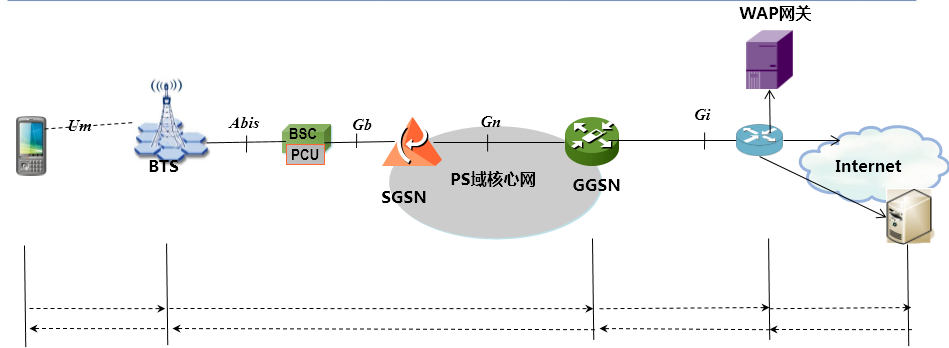
\includegraphics [width = 400pt, keepaspectratio] {mobile_to_internet.png}
    \end {figure}

    \begin {itemize}

        \item {\textcolor {blue} {MS --> BTS} }\\
        { 取决于网络情况, 2G的GPRS一般是300-600ms, EDGE在200-400ms, 3G是100ms上下, LTE则能到10-20ms. } \\

        \item {\textcolor {blue} {BTS --> GGSN} } \\
        { 这里分成了两块: BTS, BSC包括前端的MS, 都属于接入网(想想路边的大铁架子), 而后面的SGSN和GGSN这些属于运营商的分组交换域(这个是2.5G带来的设备): 这两块块网络延迟大概在1-2s左右. } \\

        \item {\textcolor {blue} {GGSN --> wap网关或者3G网关} } \\
        { 需要做协议转换, 4/7层, 处理延迟一般在30ms以下. } \\

        \item {\textcolor {blue} {wap网关或者3G网关 --> internet} } \\
        { 这属于运营商的骨干网, 如果是同运营商之间, 例如中国移动, 大概在几十ms以内, 如果跨运营商, 则由几十到上百ms. } \\

    \end {itemize}
}

\section {\ZHH 4G的普及知识} {

    {4G即是第四代移动电话行动通信标准(英语: fourth generation of mobile phone mobile communications standards, 缩写为4G), 也是3G之后的延伸. 这套无线通信标准, 从技术标准的角度看, 按照ITU的定义, 静态传输速率达到1Gbps, 用户在高速移动状态下可以达到100Mbps, 就可以作为4G的技术之一. } \\

    \vspace {6pt}
    {2G-4G的标准演进: } \\
    \begin {figure} [htbn]
        \centering
        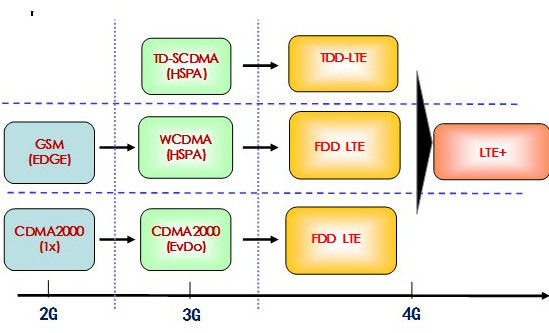
\includegraphics [width = 300pt, keepaspectratio] {4g.jpg}
    \end {figure}

    \vspace {6pt}
    { {\ZHH LTE(Long Term Evolution, 长期演进技术) } 技术便是3G的演进, 通常被称作3.9G, 包括TDD, FDD两种双工模式. TD-LTE是LTE的TDD版本, 而 FDD-LTE是LTE的FDD版本. LTE是3GPP2004年启动的项目, 分为FDD-LTE, TD-LTE, 前者由欧美主导, 后者由我国主导, 2007年工信部把TDD-LTE命名为TD-LTE. } \\

    \vspace {6pt}
    {与此对应的中国运营商: } \\
    \begin {table} [htbp]
    \centering
    \begin {tabular} {| c | c | c | c |}
        \hline
        网络标准    &   中国移动    &   中国联通    &   中国电信    \\
        \hline
        2G          &   GSM         &   GSM         &   CDMA1x      \\
        \hline
        2.5G        &   TD-SCDMA    &               &               \\
        \hline
        3G          &               &   WCDMA       &   CDMA2000    \\
        \hline
        4G          &   LTE         &               &               \\
        \hline
    \end {tabular}
    \end {table}
}

\end {document}
